\documentclass{beamer}

\title{EM Algorithm for Gaussian Mixture Model}
\author{Kai Yu}
\date{April 2013}

\usetheme{CambridgeUK}

\begin{document}

\begin{frame}
\titlepage
\end{frame}

\section{Introduction}

\begin{frame}
\frametitle{Introduction of the Guassian Mixture Model}
\framesubtitle{Recap : The Guassian distribution}
The Guassian distribution:
\begin{equation}
\mathcal{N}(x | \mu, \Sigma) = \frac{1}{(2\pi)^{D/2}}\frac{1}{|\Sigma|^{1/2}}exp\{-\frac{1}{2}(x-\mu)^T\Sigma^{-1}(x-\mu)\}
\end{equation}
\begin{figure}
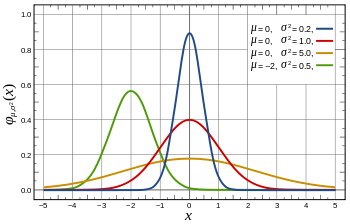
\includegraphics[width=200pt]{Guassian.png}
\end{figure}
\end{frame}

\begin{frame}
\frametitle{Introduction of the Guassian Mixture Model}
\framesubtitle{The Guassian Mixture distribution}
The Guassian Mixture distribution is a linear superposition of Guassians: 
\begin{equation}
p(x) = \Sigma^K_{k=1}\pi_k\mathcal{N}(x|\mu_k,\Sigma_k)
\end{equation}
Subject to:
\begin{equation}
\Sigma^K_{k=1}\pi_k = 1
\end{equation}
\begin{figure}
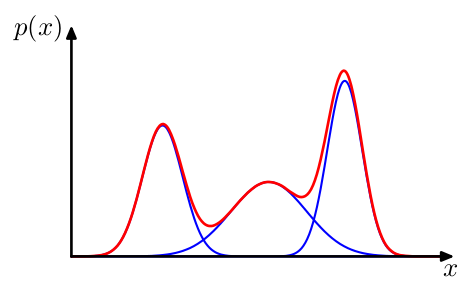
\includegraphics[width=170pt]{GMM-example2.png}\\
\end{figure}
\end{frame}

\begin{frame}
\frametitle{Introduction of the Guassian Mixture Model}
\framesubtitle{The Guassian Mixture distribution}
\begin{figure}
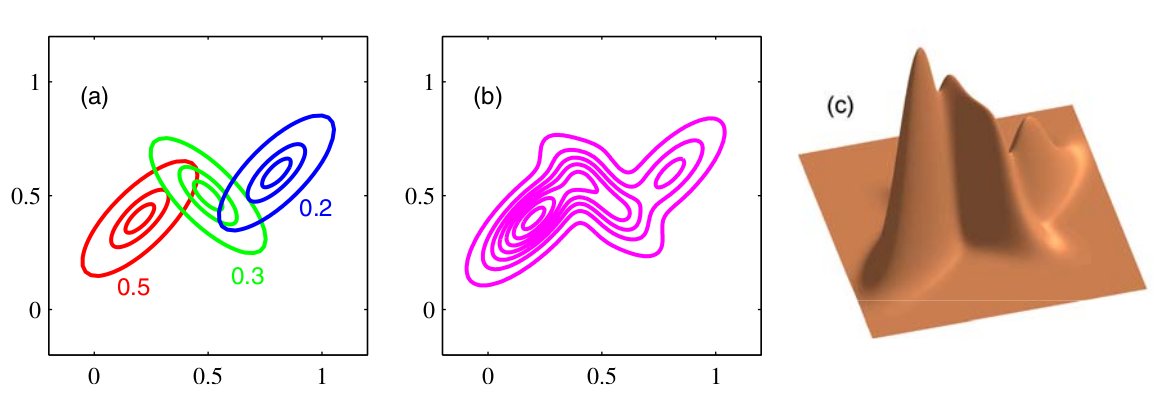
\includegraphics[width=330pt]{GMM-example.png}\\
A 2-dimension example of GMM
\end{figure}
\end{frame}

\begin{frame}
\frametitle{Introduction of the Guassian Mixture Model}
Now, for a Guassian Mixture Model, given the parameters:\\
$k$, the number of Guassian components\\
$\pi_1...\pi_k$, the mixture weights of the components\\
$\mu_1...\mu_k$, the mean of each component\\
$\Sigma_1...\Sigma_k$, the variance of each component\\
We can generate samples $s_1,s_2...s_n$ from the distribution.
\end{frame}

\begin{frame}
\frametitle{Why do we need Guassian Mixture}
\begin{figure}
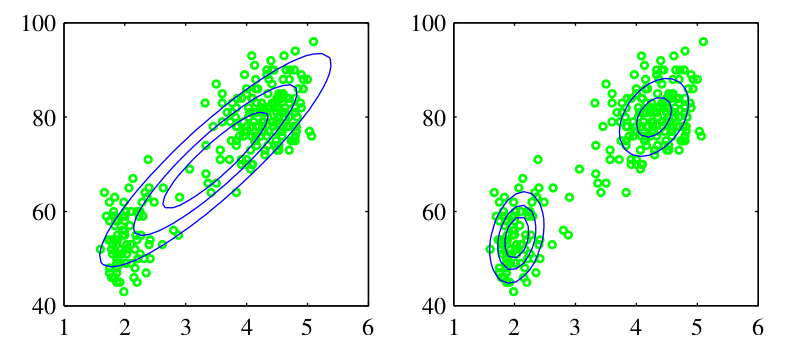
\includegraphics[width=300pt]{GMMbetterG.png}\\
In this example, we see that Guassian Mixture describes the data better a single Guassian.
\end{figure}
\end{frame}


\begin{frame}
\frametitle{The latent variable}
Given a Guassian Mixture model, we introduce K-dimensional binary random variable z which only one element $z_k$ is euqal to 1 and the others are all 0.\\
\begin{equation}
z=(0,0,..,1,0,..0)
\end{equation}
So there are K possible states for z.And we let
\begin{equation}
p(z_k=1) = \pi_k
\end{equation}
That is to say, 
\begin{equation}
p(z) = \prod^K_{k=1}{\pi_k}^{z_k}
\end{equation}
\end{frame}

\begin{frame}
\frametitle{The latent variable}
Then, we define the conditional distribution of x given a particular z:
\begin{equation}
p(x|z_k=1)=\mathcal{N}(x|\mu_k,\Sigma_k)
\end{equation}
which can also be written as:
\begin{equation}
p(x|z)=\prod^K_{k=1}{\mathcal{N}(x|\mu_k,\Sigma_k)}^{z_k}
\end{equation}
Now we can easily compute the marginal distribution of x
\begin{displaymath}
\begin{split}
p(x) = \Sigma_zp(x|z)p(z) &= \Sigma_z\prod^K_{k=1}{\mathcal{N}(x|\mu_k,\Sigma_k)}^{z_k}
\prod^K_{k=1}{\pi_k}^{z_k}\\
 &=\Sigma^K_{k=1}\pi_k\mathcal{N}(x|\mu_k,\Sigma_k)
\end{split}
\end{displaymath}
\end{frame}

\begin{frame}
\frametitle{The latent variable}
\begin{figure}
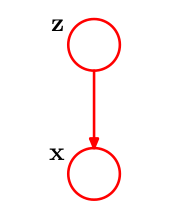
\includegraphics[width=110pt]{latent-variable.png}
\end{figure}
Now, instead of working with $p(x)$ we can work with $p(x,z) = p(x|z)p(z)$, which will lead to significant simplification when we are introducing the EM algorithm.
\end{frame}

\begin{frame}
\frametitle{The latent variable}
Another quantity $p(z|x)$ will also be very important. We use $\gamma (z_k)$ to denote $p(z_k=1|x)$, and we can use Bayes' theorem to deride its value.
\begin{equation}
\begin{split}
\gamma (z_k) = p(z_k=1|x) 
&= \frac{p(x|z_k=1)p(z_k=1)}{p(x)} \\
&= \frac{\mathcal{N}(x|\mu_k, \Sigma_k)}{\Sigma^K_{k=1}\pi_k\mathcal{N}(x|\mu_k,\Sigma_k)}
\end{split}
\end{equation}
We usually say $\gamma(z_{nk})$ is the responsibility of component k for $x_n$.
\end{frame}

\begin{frame}
\frametitle{Maximum likelihood}
Suppose we have a data set of observations $\{x_1,...,x_N\}$. And we wish to model this data set using Guassian Mixture model. We could represent this data set as an N*D matrix \textbf{X}, where N is the number of data vectors and D is the dimension of the vector. Then the log likelihood function is given by
\begin{equation}{\label{maxlike}}
lnp(X|\pi,\mu,\Sigma)=\Sigma^N_{n=1}ln\{\Sigma^K_{k=1}\pi_k
\mathcal{N}(x_n|\mu_k,\Sigma_k)\}
\end{equation}
\end{frame}

\begin{frame}
\frametitle{E-M algorithm for Gaussian mixtures}
The expectation-maximization algorithm is an elegant and powerful method for finding maximum likelihood solutions for models with latent variables.\\
First, we set the derivatives of $lnp(X|\pi,\mu,\Sigma)$ in equation \ref{maxlike} with repect to $\mu_k$ to zero.
\begin{equation}
\begin{split}
0&=-\Sigma^N_{n=1}\frac{\pi_k\mathcal{N}(x_n|\mu_k,\Sigma_k)}{\Sigma^K_{j=1}\pi_j
\mathcal{N}(x_n|\mu_j,\Sigma_j)}\Sigma_k(x_n-\mu_k)\\
&=-\Sigma^N_{n=1}\gamma(z_{nk})\Sigma_k(x_n-\mu_k)
\end{split}
\end{equation}
If we assume $\Sigma_k$ to be nonsingular, we obtain
\begin{equation}{\label{m1}}
\mu_k=\frac{\Sigma^{N}_{n=1}\gamma(z_{nk})x_n}{\Sigma^{N}_{n=1}\gamma(z_{nk})}
\end{equation}
\end{frame}

\begin{frame}
\frametitle{E-M algorithm for Gaussian mixtures}
We set $N_k=\Sigma^{N}_{n=1}\gamma(z_{nk})$, as the effective number of points assigned to cluster k.\\
If we set the derivative of $lnp(X|\pi,\mu,\Sigma)$ with respect to $\Sigma_k$ to zero,we get
\begin{equation}{\label{m2}}
\Sigma_k=\frac{1}{N_k}\gamma_k(z_{nk})(x_n-\mu_k)(x_n-\mu_k)^T
\end{equation}
\end{frame}


\begin{frame}
\frametitle{E-M algorithm for Gaussian mixtures}
Finally, when we maximize the log likelihood with respect to $\pi$, we need to take the constraint $\Sigma_{k=1}^K\pi_k=1$ into consideration.
This is done by using the Lagrange multiplier.
\end{frame}

\begin{frame}
\begin{block}{The Lagrange Multiplier}
We want to maximize $f(x,y)$ subject $g(x,y) = c$.\\
Let $\Lambda(x, y \lambda) = f(x,y) + \lambda (g(x,y)-c)$.Then if $(x_0, y_0)$is a maximum of the original $f$, there exists $(x_0,y_0,\lambda_0)$ is a stationary point for the $\Lambda$ function.\\
\begin{figure}[L]
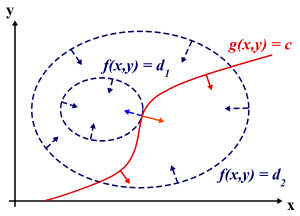
\includegraphics[width=130pt]{Lagrange.png}
\end{figure}
The contour lines of f and g touch when the tangent vectors of the contour lines are parallel. Since the gradient of a function is perpendicular to the contour lines, this is the same as saying that the gradients of f and g are parallel. 
\end{block}
\end{frame}

\begin{frame}
\begin{block}{The Lagrange Multiplier}
So $\nabla_{x,y}f =  - \lambda \nabla_{x,y}g$.\\
Combining with the constraint, we get $\nabla_{x,y,\lambda}\Lambda = 0$
\end{block}
Now, we apply the Lagrange Multiplier to maximize with respect to $\pi$. We will be maximizing
\begin{equation}
lnp(x|\pi,\mu,\Sigma)+\lambda(\Sigma_{k=1}^K\pi_k-1)
\end{equation}
By maximizing it we will get 
\begin{equation}{\label{m3}}
\pi_k=\frac{N_k}{N}
\end{equation}
\end{frame}

\begin{frame}
\frametitle{E-M algorithm for Gaussian mixtures}
We have to note that the solutions \ref{m1}, \ref{m2}, \ref{m3} are not closed. Because the responsibilities $\gamma(z_{nk})$ depend on the parameters. However, they suggest a iterative scheme for finding a solution to the maximum likelihood problem. 
\end{frame}
\begin{frame}
\frametitle{E-M algorithm for Gaussian mixtures}

\textbf{Initialize} Initialize the parameters $\mu_k$, $\Sigma_k$, and $\pi_k$\\
\textbf{E-step} Evaluate the responsibilities using the current parameter values.
\begin{equation}
\begin{split}
\gamma (z_{nk}) = \frac{\mathcal{N}(x_n|\mu_k, \Sigma_k)}{\Sigma^K_{k=1}\pi_k\mathcal{N}(x_n|\mu_k,\Sigma_k)}
\end{split}
\end{equation}

\end{frame}

\begin{frame}
\frametitle{E-M algorithm for Gaussian mixtures}
\textbf{M-step} 
Re-estimate the parameters using the current responsibilities.
\begin{equation}
\begin{split}
\mu_k^{new}&=\frac{1}{N_k}{\Sigma^{N}_{n=1}\gamma(z_{nk})x_n}\\
\Sigma_k^{new}&=\frac{1}{N_k}\gamma_k(z_{nk})(x_n-\mu_k)(x_n-\mu_k)^T\\
\pi_k^{new}&=\frac{N_k}{N}
\end{split}
\end{equation}
\textbf{Likelihood} Recalculate the log likelihood function to see if it converges, if not, go to step 1 again.
\end{frame}

\begin{frame}
\frametitle{An Example}
\begin{figure}
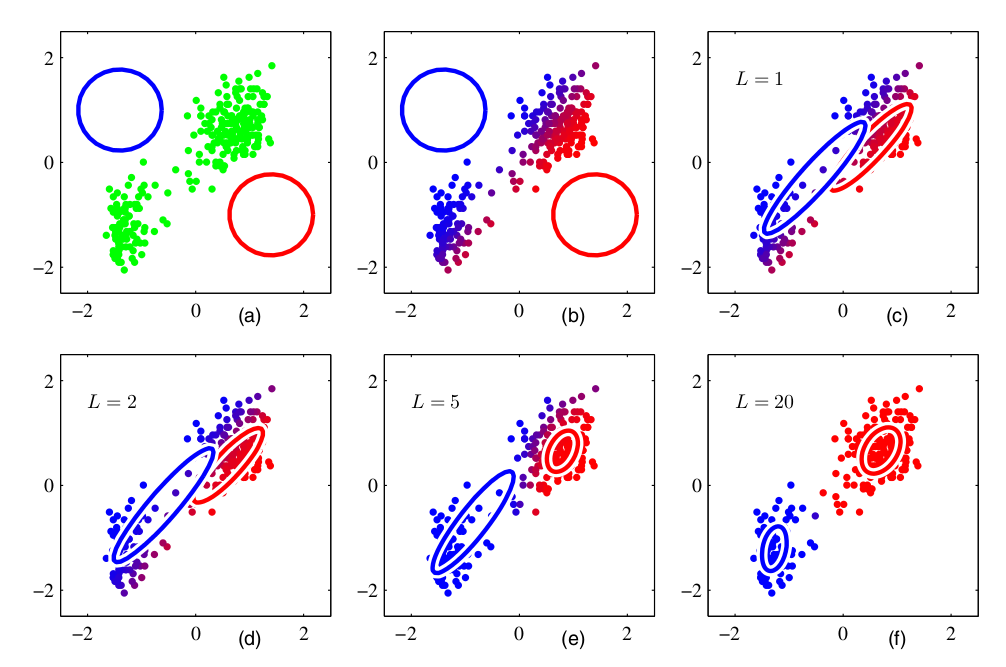
\includegraphics[width=300pt]{EM-example.png}
\end{figure}
\end{frame}

\begin{frame}
Now we've know the inituition of the EM algorithm, and we are going to proof its property. We will need the Jensen Inequality.
\begin{block}{Jensen's Inequality}
If $X$ is a random variable and $\varphi$ is a convex function.
Then $\varphi(E[X]) \leq E[\varphi(X)]$.
\begin{figure}
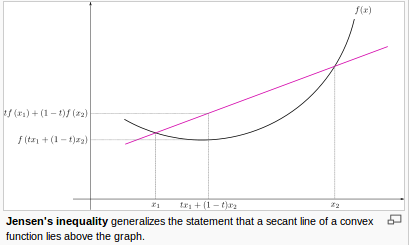
\includegraphics[width=200pt]{jensen.png}
\end{figure}
\end{block}
\end{frame}

\begin{frame}
\frametitle{The General EM}
\begin{block}{Theorem}
In each iteration, the E-M algorithm gives a solution that gives higher likelihood.
\end{block}
\emph{Proof:}For simplicity, we denote all parameters as $\theta$.
Remembering the latent variable $Z$, we can now write the log likelihood as
\begin{equation}
lnp(X|\theta)=ln\{\Sigma_zp(X,z|\theta)\}
\end{equation}
In the E-step, we are are actually forming an ancillary function(go back to \ref{m1}, \ref{m2}, \ref{m3} and check it):
\begin{equation}
\mathcal{Q}(\theta,\theta^{old})=\Sigma_zp(z|X,\theta^{old})lnp(X,z|\theta)
\end{equation}
Then, in the M-step, we are maximizing $\mathcal{Q}(\theta,\theta^{old})$, and get the $\theta^{new}$.
\end{frame}

\begin{frame}
\frametitle{The General EM}
Now we use Jensen's inequality to transform the log likelihood function.
\begin{equation}{\label{anci}}
\begin{split}
lnp(X|\theta) &= ln\{\Sigma_z\frac{q(z)p(X,z|\theta)}{q(z)}\}\\
&\geq \Sigma_zq(z)ln(\frac{p(X,z|\theta)}{q(z)})\\
&=\Sigma_zq(z)ln(p(X,z|\theta))-\Sigma_zq(z)ln(q(z))
\end{split}
\end{equation}
To continue we need to prove a lemma first.
\end{frame}
\begin{frame}
\begin{block}{lemma}
If $q(z)=p(z|\theta,X)$, equation \ref{anci} becomes an equality.\\
\emph{Proof:}
\begin{equation}
\begin{split}
lnp(X|\theta)- \Sigma_zq(z)ln(\frac{p(X,z|\theta)}{q(z)})\\
=\Sigma_zq(z)\{ln(p(X|\theta))-ln(\frac{p(X,z|\theta)}{q(z)})\}\\
=\Sigma_zq(z)\{ln(\frac{q(z)}{p(z|\theta,X)})\}\\
=\Sigma_zq(z)ln(1)=0
\end{split}
\end{equation}
\end{block}
\end{frame}

\begin{frame}
\frametitle{The General EM}
\framesubtitle{completing the proof}
Now we let $q(z)=p(z|X,\theta^{old})$, then we can complete our proof.
\begin{equation}
\begin{split}
ln(p(X|\theta^{new}) &\geq \Sigma_zq(z)ln(p(X,z|\theta^{new}))-\Sigma_zq(z)ln(q(z))\\
&=\mathcal{Q}(\theta^{new}, \theta^{old})- \Sigma_zq(z)ln(q(z))\\
&\geq \mathcal{Q}(\theta^{old}, \theta^{old})- \Sigma_zq(z)ln(q(z))\\
&= ln(p(X|\theta^{old})
\end{split}
\end{equation}
\end{frame}
\section*{Bibliography}
\begin{frame}%[allowframebreaks] % add this if you have more papers to cite than fit on a slide.
\frametitle{Bibliography}

\begin{thebibliography}{Tantau, 2007}
\bibitem[aaPicutre]{Beamer}
Some pictures are from Wiki or PRML

\end{thebibliography}
\end{frame}
\end{document}
